\chapter{Охрана труда}

\section{Анализ условий труда на рабочем месте аналитика в НИЛ}

Производственное помещение, научно-исследовательская лаборатория (НИЛ), содержит
одно рабочее место, которое включает:

\begin{itemize}

    \item 2 ПК в комплектации: системный блок, жидкокристаллический экран, мышь, клавиатура;

    \item WiFi роутер.

\end{itemize}

Размеры помещения составляют 2,5х3х3 (м). Нормой, в соответствии с ДСан ПиН
3.3.2-007-98, является площадь на одно робочее место не менее 6,0 (кв. м) объём
--- не менее 20,0 (куб. м). Помещение НИЛ включает 1 рабочее место площадью 7,5
(кв. м) и объёмом 22,5 (куб. м).

С целью анализа условий труда в помещении НИЛ была рассмотрена система
"Человек-Машина-Среда" (Ч-М-С).

Ч1 --- аналитик, который выполняет работу на ПК.

Ч2 --- аналитик, который рассматривается с точки зрения влияния на окужающую
среду.

Ч3 --- психофизиологическое состояние человека.

М1 --- ПК, используемый аналитиком.

М2 --- аварийная защита ПК.

М3 --- влияние ПК на окружающую среду и человека.

Среда --- внутренняя среда помещения: освещение, микроклимат.

ПТ --- предмет труда --- анализ возможных атак в протоколе WEP.

Структура системы Ч-М-С рассмотрена на рисунке~\ref{fig:worker_safety_HME}.
Направление и содержание связей сведены в таблицу~\ref{table:worker_safety_HME}

\begin{figure}
    \begin{center}
       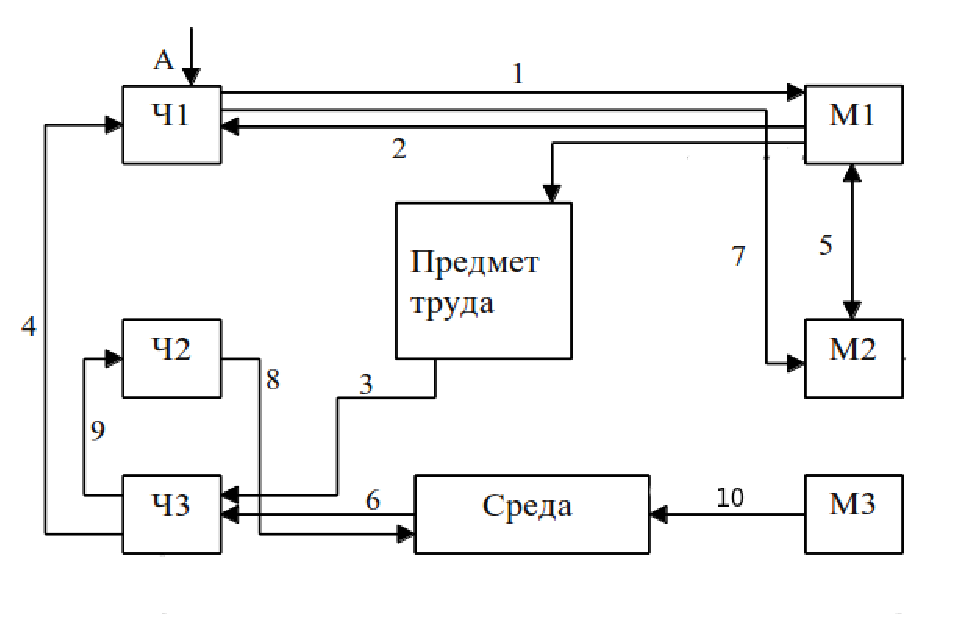
\includegraphics[width=100mm]{graphics/worker_safety_HME.eps}
    \end{center}
    \caption{Cтруктура системы Ч-М-С}
    \label{fig:worker_safety_HME}
\end{figure}

\begin{table}
    \caption{Декомпозиция системы Ч-М-С.}
    \label{table:worker_safety_HME}
    \begin{tabular}{| m{1.3cm} | m{2cm} | m{11.7cm} |}
        \hline
        Номер связи & Направ- ления связи & Содержание связи                                                                                           \\ \hline
        1           & Ч1-М1              & Влияние человека на ПК и его настройки                                                                     \\ \hline
        2           & М1-Ч1              & Информация про состояние ПК                                                                                \\ \hline
        3           & ПТ-Ч3              & Влияние процесса анализа атак на психологическое состояние аналитика                                       \\ \hline
        4           & Ч3-Ч1              & Уменьшение продуктивности работы вследствие монотонности труда и умственного перенапряжения                \\ \hline
        \multirow{2}{*}{5} & М1-М2       & Информация, необходимая для генерации аварийного управляющего влияния                                      \\ \cline{2-3}
                           & М2-М1       & Недостаточная освещённость и вентиляция рабочего места                                                     \\ \hline
        6           & С-Ч3               & Влияние среды на состояние организма аналитика                                                             \\ \hline
        7           & Ч1-М2              & Влияние аналитика на аварийное состояние ПК                                                                \\ \hline
        8           & Ч2-С               & Выделения углекислого газа вследствие процесса дыхания, выделение тепла и пота                             \\ \hline
        9           & Ч3-Ч2              & Влияние психофизиологического состояния на степень интенсивности обмена веществ между организмом и средой  \\ \hline
        10          & М3-С               & Электромагнитные излучения, шум, температура                                                               \\ \hline
    \end{tabular}
\end{table}

Потенциально опасными и вредными производственнми факторами по ГОСТ 12.0.003-74
для данного помещения НИЛ являются:

\begin{enumerate}

    \item физические:

    \begin{itemize}

        \item повышенная или пониженная температура воздуха рабочей зоны;
        
        \item повышенная или пониженная подвижность воздуха;
        
        \item отсутствие или недостаток естественного света;
        
        \item недостаточная освещённость рабочей зоны;
        
    \end{itemize}

    \item химические: отсутствуют;
   
    \item биологические: отсутствуют;
    
    \item психофизиологические:

    \begin{itemize}

        \item монотонность труда;

        \item умственное перенапряжение;

        \item перенапряжение анализаторов (зрительные).

    \end{itemize}

\end{enumerate}

Доминирующим вредным производственным фактором является недостаток естественного
света.


\section{Промышленная безопасность в производственном помещении НИЛ}

Характеристики сети электропитания: трёхфазная четырёхпроводная сеть переменного
тока с глухозаземлённой нейтралью и напряжением 380/220 В, частотой 50 Гц.
Согласно НПАОП 40.1-1.21-98 помещение по опасности поражения электрическим током
относится к классу без повышенной опасности.

В помещении отсутствуют другие опасные производственные факторы.

Для защиты людей от поражения электрическим током предусмотрено зануление,
двойная изоляция, защитное отключение устройств в помещении (согласно ГОСТ
12.1.033-81).

Для обеспечения безопасности работы проводится вводный, первичный и повторный (1
раз в 6 месяцев) иствруктажи по технике безопасности (согласно НПАОП
0.00-4.12.05).

\section{Производственная санитария в помещении НИЛ}

Работы в помещении согласно ГОСТ 12.1.005-88 относятся к категории работ с
энергозатратами организма "лёгкая 1а" - сидячая работа, не требует
систематического физического напряжения и перемещения предметов с
энергозатратами организма 90-120 кКал/час.

Для обеспечения установленных норм микроклиматических параметров и чистоты
воздуха используется кондиционирование воздуха в тёплый период и отопление в
холодный.

В светлое время суток рекомендуется использовать естественное освещение, а
искустенное только в условиях недостаточности естественного освещения. Для
искуственного освещения используют люминисцентные лампы за счёт их высокой
световой отдачи, длительного срока службы, экономности и более близкому к
ествественному спектру.

Определяем нормированное значение коэффициента естественной освещенности (КЕО)
$e^{III}_n$ для выполняемой зрительной работы. В соответствии с исходными
данными наименьший объект различения --- толщина хромирующего покрытия,
характеристика зрительной работы --- Наивысшей точности, I разряд, подразряд а.
Для территории Украины без устойчивого снежного покрова значение $e^{III}_n =
2\%$.

Вычисляем КЕО для данного светового климата в соответствии со следующей
формулой:
$$e^{I,II,III,IV}_n = e^{III}_n m C,$$
где $e^{III}_n$ --- значение КЕО для зданий, расположенных в III поясе светового
климата; $m$ --- коэффициент светового климата; $C$ --- коэффициент солнечности
климата.

Город Харьков расположен в IV поясе светового климата, для которого (при
заданном в условии диапазоне азимута $m = 0,9$) $C = 1$. Тогда $e^{IV}_n = 1,8\%$.

Коеффициент естественного освещения равен 1,8\%, что удовлетворяет ДСН
В.2.5-28-2006.

\section{Пожарная безопасность производственного помещения НИЛ}

Производство, включающее научно-исследовательскую лабораторию, имеет категорию Д
пожаровзрвыоопасности, согласно НАПБ Б.03.002-2007. Степень огнестойкости здания
--- II, согласно ДБН В.1.1.7-2002, так как помещение расположено в кирпичном
здании, при строительстве использовались твёрдые несгораемые материалы.

Возможные причины возникновения пожара на рабоем месте или в помещении:

\begin{itemize}

    \item короткое замыкание, сопровождающееся искрением и перегревом элементов
    ПК вследствие чего происходит воспламенение оборудования;

    \item перегрев элементов ПК в следствии высокой нагрузки во время проведения
    атаки;

    \item кабели для подачи электропитания.

\end{itemize}

В помещении присутствуют два углекислотных огнетушителя ВВК-1,4, при норме 2
огнетушителя на 20 кв.м, согласно НПАОП 0.00-1.28-10.

Эвакуация производится по плану эвакуации, по центральной лестнице, через
главный выход. Дополнительный эвакуационный выход отсутствует так как в
помещении работает 1 человек и площадь помещения составляет 7,5 кв.м.

